\section{Integer matching and allocation}
\label{sec:allocation}

Globex supports several matching families. FIFO, pro rata, TOP, LMM, and configurable combinations have different roles; the assigned product configuration determines which stages apply. A generic ``CME pro-rata formula'' is therefore insufficient. The public algorithm matrix supplies the order of stages, while the step documentation specifies their local behavior \citep{CMEMatching,CMESteps}.

\subsection{Price selection and allocation are different maps}

Let a buy aggressor have remaining size $Q$ and limit $L$. First identify the best eligible opposite price, including eligible implication. At a selected price, let $q=(q_1,\ldots,q_n)$ be the quantities available to the relevant allocation stage. The stage produces
\begin{equation}
 f=\mathcal A(q,y;\vartheta),\qquad
 0\le f_i\le q_i,\quad \sum_i f_i\le y,
\end{equation}
where $\vartheta$ contains that stage's configuration and $y$ is its available aggressor quantity. A later stage operates on updated remaining quantities. The proportions in a later pro-rata step must therefore use its own input state, rather than the original book automatically.

For a declared stage with sufficient compatible resting quantity, complete allocation requires $\sum_i f_i=y$. The public step description also identifies a FIFO exception when aggressing quantity exceeds available resting quantity. In the ordinary displayed examples here, that exception exhausts the available orders. We do not model the ordering of individual execution reports in that branch.

\subsection{FIFO as a prefix operator}

Order the eligible ordinary orders first by best price and then by applicable time priority. Define $H_i=\sum_{j\le i}q_j$, with $H_0=0$. The FIFO fill is
\begin{equation}
 f_i(Q)=\min\{q_i,(Q-H_{i-1})_+\}.
\label{eq:fifo}
\end{equation}

\begin{proposition}[FIFO conservation and composition]\label{prop:fifo}
Under Assumption~\ref{ass:scope}, FIFO fills $\min(Q,H_n)$ contracts and never fills a later order while leaving available quantity ahead of it. Two consecutive aggressors with the same side and limit, sizes $Q_1,Q_2$, and no intervening state change have the same total order-level fills as one aggressor of size $Q_1+Q_2$.
\end{proposition}
\begin{proof}
Represent order $i$ by the interval $(H_{i-1},H_i]$ on a quantity axis. Its fill is the length of its intersection with $(0,Q]$. The intersections partition $(0,\min(Q,H_n)]$, establishing conservation and priority. The first aggressor removes a prefix. The second removes the next prefix of the residual list. Their union is the prefix of length $\min(Q_1+Q_2,H_n)$.
\end{proof}

The interval argument fails if a new event refreshes hidden display, changes priority, or elects additional interest. CME's FIFO modification documentation identifies working-size increases, price changes, and account-number changes as priority-losing amendments \citep{CMESteps}. The composition statement deliberately excludes amendments and replenishment.

\subsection{A pro-rata stage with an integer minimum}

We now specify one complete model: a pro-rata step with integer minimum $h\ge1$, followed by ordinary FIFO residual allocation, with no TOP, LMM, split, or leveling step. Working quantities mean eligible displayed quantities in this model. Let
\begin{equation}
 Q_0=\sum_iq_i>0,\qquad 0\le y\le Q_0,\qquad
 w_i=\frac{yq_i}{Q_0}.
\end{equation}
The first-pass allocation and residual are
\begin{equation}
 b_i=\begin{cases}\lfloor w_i\rfloor,&\lfloor w_i\rfloor\ge h,\\
 0,&\lfloor w_i\rfloor<h,
 \end{cases}
 \qquad \rho=y-\sum_i b_i.
\label{eq:prbase}
\end{equation}
Apply FIFO to residual capacities $q_i-b_i$ with size $\rho$ to obtain $r_i$; finally $f_i=b_i+r_i$. Thresholding the integer part is equivalent to testing $w_i\ge h$ because $h$ is an integer. This model follows the documented minimum-and-rounding structure \citep{CMESteps}, but is not an implementation of every supported algorithm.

\begin{proposition}[Conservation and discrepancy]\label{prop:rounding}
The above allocation is well defined and satisfies
\begin{equation}
 \sum_i f_i=y,\quad 0\le f_i\le q_i,\quad
 0\le\rho<nh,\quad
 \sum_i|f_i-w_i|\le2\rho<2nh.
\end{equation}
\end{proposition}
\begin{proof}
Since $y\le Q_0$, $b_i\le w_i\le q_i$. If $b_i=0$, then $0\le w_i<h$. Otherwise $0\le w_i-b_i<1\le h$. Summing gives $\rho=\sum_i(w_i-b_i)\in[0,nh)$. Residual capacity is $Q_0-\sum_i b_i\ge\rho$, so FIFO allocates the entire residual without exceeding capacity. Write $d_i=w_i-b_i\ge0$. Then $f_i-w_i=r_i-d_i$, with $\sum_i r_i=\sum_i d_i=\rho$. The triangle inequality gives the claimed bound.
\end{proof}

This is a bound on departure from the fractional allocation of a \emph{single stage}. It is not a guarantee that final allocations of a multi-stage algorithm are approximately proportional. A priority stage may intentionally allocate a large fraction to one order. When $y=Q_0$, the final vector is $q$ regardless of how the intermediate rounding is organized.

\begin{table}[htbp]
\centering
\begin{tabular}{@{}lrrrrr@{}}
\toprule
Order & Resting size & Fractional $w_i$ & PR base & PR + FIFO & FIFO\\
\midrule
1 & 12 & 4.44 & 4 & 5 & 12\\
2 & 28 & 10.36 & 10 & 10 & 25\\
3 & 60 & 22.20 & 22 & 22 & 0\\
\midrule
Total & 100 & 37.00 & 36 & 37 & 37\\
\bottomrule
\end{tabular}
\caption{A 37-contract aggressor at one price, $h=2$, and orders listed in FIFO order. All prices are identical, so allocation changes who fills without changing this aggressor's execution price.}
\label{tab:allocation}
\end{table}

\subsection{Fragmentation changes the mechanism's input}

\begin{example}[No general event-composition law]\label{ex:fragment}
Take $q=(2,3,5)$ and $h=2$. For a single aggressor of size four, $w=(0.8,1.2,2)$, the PR base is $(0,0,2)$, and the two residual contracts go to the first order. Thus $f=(2,0,2)$.

Instead submit two consecutive aggressors of size two. On the first, no fractional entitlement reaches two, so FIFO allocates $(2,0,0)$. Remaining sizes are $(0,3,5)$. On the second, entitlements are $(0,0.75,1.25)$, again all below two. FIFO gives $(0,2,0)$. Total fills are $(2,2,0)$.
\end{example}

The difference is caused by the reset of the proportional calculation at the next event. A simulator that merges the two aggressors changes the result even though total quantity, side, and price are unchanged. Similarly, replacing the $h=2$ minimum by $h=1$ in the single-event example gives $(1,1,2)$ rather than $(2,0,2)$.

\begin{figure}[htbp]
\centering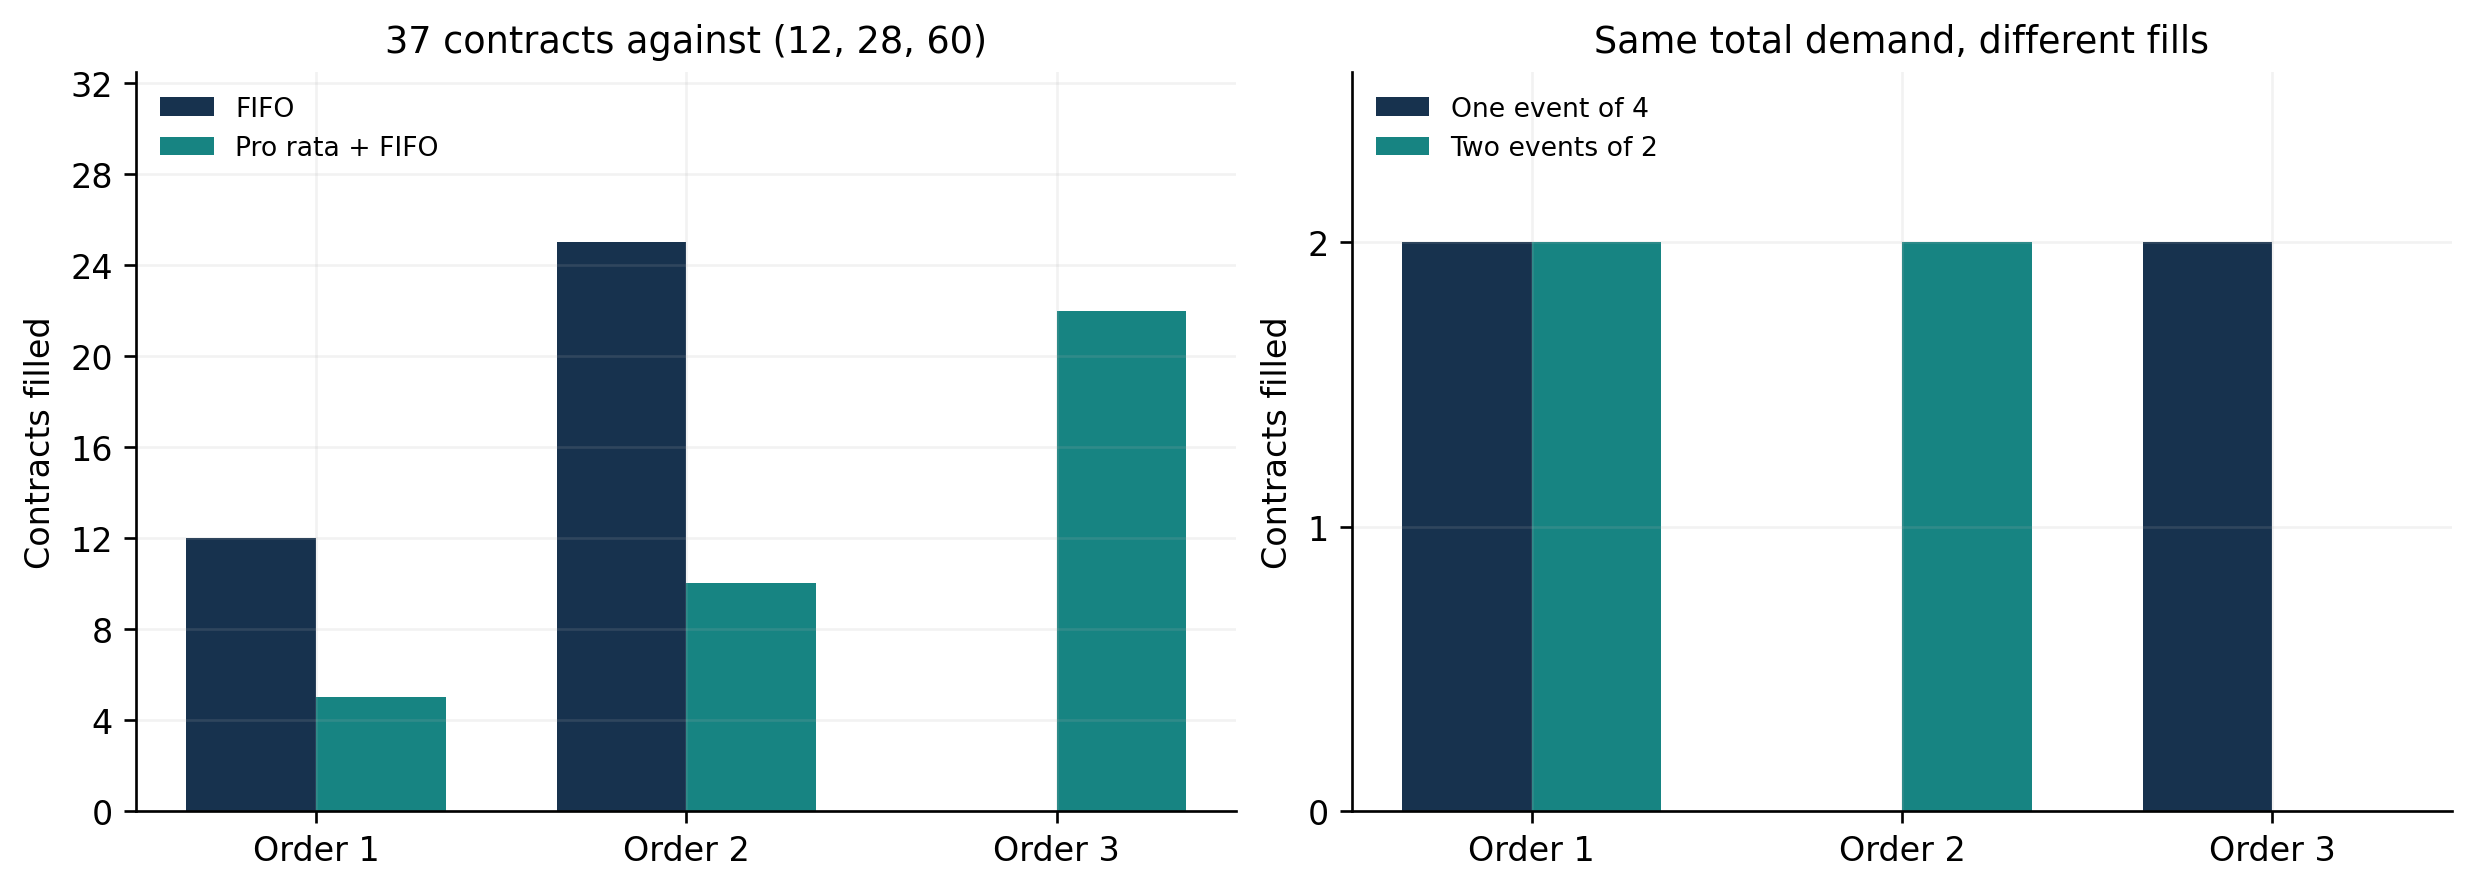
\includegraphics[width=\textwidth]{figures/01_allocation.png}
\caption{Allocation effects isolated from price effects. Left: Table~\ref{tab:allocation}. Right: Example~\ref{ex:fragment}. Contract conservation holds in every bar group; participant outcomes differ.}
\label{fig:allocation}
\end{figure}

\subsection{What a configurable model must preserve}

It is useful to write a configured allocator as a composition of stages, but the composition operates on both remaining demand and remaining book state:
\begin{equation}
 (q^{k+1},y^{k+1},\eta^{k+1})
 =T_k(q^k,y^k,\eta^k),
\end{equation}
where $\eta$ contains entitlement and priority information. Stage order, eligibility, integer rounding, and residual handling are all part of $T_k$. The configurable family includes optional leveling after proportional allocation; it must not be silently replaced by the FIFO residual model above \citep{CMEMatching}. We do not assign undocumented entitlement percentages to a named product.

The right abstraction is therefore a family of allocation maps indexed by configuration and market phase. Contract conservation survives across the family when each stage is conservative. FIFO composition and proportional discrepancy bounds require their additional assumptions.
\FloatBarrier
